\newpage

\section{EAR - Eye Aspect Ratio} \label{section:EARsection}

Metoda polegająca na obliczeniu \textit{EAR}  \cite{EARRaspberryPi} \cite{eyeBlinkEARRosebrock}, czyli stosunek otwarcia oczu - wysokość do szerokości widocznej części gałki ocznej. Wykorzystuje się tu facemarki (patrz rozdz. \hyperref[{section:landmarks}]{\textit{\ref{section:landmarks}.Facemarks}}) naniesione dookoła oczu.

\subsection{Wzór obliczania EAR}
Zależnie od ilości punktów wokół oka będzie różny wzór obliczania EAR.\\
Dla 6 punktów:
\begin{align}
    EAR = \frac{dist(L_0, L_1) + dist(L_2, L4)}{2 * dist(L_3, L_5)}
\end{align}
\\
Natomiast, dla 4 punktów:
\begin{align}
    EAR = \frac{dist(L_0, L_2)}{dist(L_1, L_3)}
\end{align}

Gdzie \textit{$L_x$} to kolejne landmarki dokoła oczu, a \textit{dist} to odległość między dwoma punktami (odległość euklidesowa).\\

\subsection{Zasada działania EAR w kontekście mrugania i określenia czy oko jest otwarte/zamknięte}

W teorii otwarte oczy będą miały większy wymiar liczbowy EAR, niż oczy zamknięte. Na \hyperref[{fig:theoretical_eye_landmarks}]{\textit{rysunku \ref{fig:theoretical_eye_landmarks}}} widać, że oko otwarte ma większe odległości między punktami pionowymi niż w przypadku oka zamkniętego. Dzięki takim różnicą możemy wykryć spadek wskaźnika EAR poniżej pewnego ustalonego poziomu, oznaczający zamknięcie oka, natomiast wzrost, otwarcie oka. Całościowo obserwując zmiany np. za pomocą pochodnej jesteśmy w stanie stwierdzić mrugnięcie.

\begin{figure}[!h]
    \begin{center}
        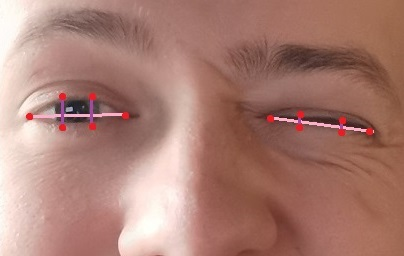
\includegraphics[scale=0.35]{img/landmark_section/theoretical_eye_landmarks.jpg}
        \caption{Teoretyczny rozmieszczene landmarków wokół oczu wraz z naniesionymi połączeniami do obliczenia EAR}
        \label{fig:theoretical_eye_landmarks}
    \end{center}
\end{figure}


\subsection{Wyznaczenie progu EAR}

Korzystając z tej metody potrzebujemy określić pewien próg wskaźnika EAR, poniżej którego będziemy klasyfikować oczy jako zamknięte lub mrugające. W tym celu zebrałem dane dotyczące wyliczonego stosunku zarówno na statycznych zdjęciach, jak i obrazie na żywo.

\subsubsection{Statyczne zdjęcia}

Na podstawie używanego datasetu wyliczyłem EAR dla wszystkich oczu i podzieliłem je na dwie grupy: oczy otwarte (rys. \ref{fig:ear_static_open}) i oczy zamknięte (rys. \ref{fig:ear_static_close}). 

\vspace{5mm}

\begin{figure}[!h]
    \centering
    \begin{tikzpicture}
        \begin{axis}[
            ylabel = {EAR},
            height = 0.4\linewidth,
            width = \linewidth,
            ymin= {0.10},
            ymax={0.40},
            ytick = {0.10, 0.15, 0.20, 0.25, 0.30, 0.35},
            xticklabel = \empty,
            xtick = \empty,
            ymajorgrids = {true},
        ]
            \addplot[color=blue, mark=square*] table [x=x, y=ear, col sep=comma] {csv/ear_static_open.csv};
        \end{axis}
    \end{tikzpicture}
    \caption{EAR dla oczu otwartych}
    \label{fig:ear_static_open}
\end{figure}

\begin{figure}[!h]
    \centering
    \begin{tikzpicture}
        \begin{axis}[
            ylabel = {EAR},
            height = 0.4\linewidth,
            width = \linewidth,
            ymin= {0.10},
            ymax={0.25},
            ytick = {0.1, 0.15, 0.2, 0.25},
            xticklabel = \empty,
            xtick = \empty,
            ymajorgrids = {true},
        ]
            \addplot[color=blue, mark=square*] table [x=x, y=ear, col sep=comma] {csv/ear_static_closed.csv};
        \end{axis}
    \end{tikzpicture}
    \caption{EAR dla oczu zamkniętych}
    \label{fig:ear_static_close}
\end{figure}

W przypadku oczu otwartych widać, że poza kilkoma wyjątkami wskaźnik EAR znajduje się powyżej $0.20$, a czasem przekraczając nawet $0.35$. Przypadek gdzie wartość  jest poniżej $0.15$ wynika najprawdopodobniej z faktu, że oczy były mocno przymknięte i ze względu na perspektywę rozciągnięte horyzontalnie. Odchylenie takie traktuję jako przypadek skrajny i nie wpływający na wyniki.
\par
Na wykresie dla oczu zamkniętych ponownie próg zdaje się być na poziomie $0.20$, a większość wskaźników osiąga wartość około $0.19$. 

\subsubsection{Obraz z kamery}

Na obrazie z kamery urządzenia przeprowadziłem trzy testy wskaźnika EAR: oczy otwarte (rys. \ref{fig:ear_live_open}), oczy chwilowo zamknięte (rys. \ref{fig:ear_live_close}) oraz mrugnięcie (rys. \ref{fig:ear_live_blink}). na wykresach czerwony kolor oznacza EAR dla prawego oka, natomiast niebieski dla lewego.


\begin{figure}[!h]
    \centering
    \begin{tikzpicture}
        \begin{axis}[
            xlabel = {Nr klatki obrazu z kamery},
            ylabel = {EAR},
            height = 0.4\linewidth,
            width = \linewidth,
            ymin= {0.20},
            ymax={0.35},
            ytick = {0.20, 0.25, 0.30, 0.35},
            ymajorgrids = {true},
        ]
            \addplot[color=blue, mark=square*] table [x=x, y=left, col sep=comma] {csv/ear_live_open.csv};
            \addplot[color=red, mark=square*] table [x=x, y=right, col sep=comma] {csv/ear_live_open.csv};
        \end{axis}
    \end{tikzpicture}
    \caption{Oczy otwarte na obrazie z kamery}
    \label{fig:ear_live_open}
\end{figure}

W tym przypadku oczy były przez cały czas otwarte. Liczbowy wymiar EAR nie spadał poniżej $0.25$, a przez większość czasu trzymał się nawet powyżej $0.30$.

\begin{figure}[!h]
    \centering
    \begin{tikzpicture}
        \begin{axis}[
            xlabel = {Nr klatki obrazu z kamery},
            ylabel = {EAR},
            height = 0.4\linewidth,
            width = \linewidth,
            ymin= {0.10},
            ymax={0.35},
            ytick = {0.15, 0.20, 0.25, 0.30, 0.35},
            ymajorgrids = {true},
        ]
            \addplot[color=blue, mark=square*] table [x=x, y=left, col sep=comma] {csv/ear_live_close.csv};
            \addplot[color=red, mark=square*] table [x=x, y=right, col sep=comma] {csv/ear_live_close.csv};
        \end{axis}
    \end{tikzpicture}
    \caption{Oczy czasowo zamknięte na obrazie z kamery}
    \label{fig:ear_live_close}
\end{figure}

W tym teście oczy były czasowo zamknięte. Najpierw w przedziale klatek $[25, 60]$ zamknięte było tylko oko prawe, następnie w przedziale $[80,120]$ tylko lewe, a na końcu w okresie $[140,190]$ oba oczy jednocześnie. Zmiana EAR jest tutaj mocno wyraźna, a w~tych trzech przedziałach miał wartość między $0.10$, a $0.20$. Dodatkowo na podstawie tych danych trzeba również odnotować spadek EAR dla obu oczu nawet w przypadku zamknięcia tylko jednego. Może to wynikać z faktu, że człowiek zamykając jedno przymyka lekko również drugie. Ale przyczyną może być też sam algorytm facemarków, w którym punkty dla różnych oczu mogą być ze sobą skorelowane.

\begin{figure}[!h]
    \centering
    \begin{tikzpicture}
        \begin{axis}[
            xlabel = {Nr klatki obrazu z kamery},
            ylabel = {EAR},
            height = 0.4\linewidth,
            width = \linewidth,
            ymin= {0.10},
            ymax={0.35},
            ytick = {0.15, 0.20, 0.25, 0.30, 0.35},
            ymajorgrids = {true},
        ]
            \addplot[color=blue, mark=square*] table [x=x, y=left, col sep=comma] {csv/ear_live_blink.csv};
            \addplot[color=red, mark=square*] table [x=x, y=right, col sep=comma] {csv/ear_live_blink.csv};
        \end{axis}
    \end{tikzpicture}
    \caption{Mruganie na obrazie z kamery}
    \label{fig:ear_live_blink}
\end{figure}

W trzeciej wariacji testu na obrazie z kamery występowały mrugnięcia: w przedziale $[30,40]$ prawego oka, $[55,65]$ lewego, a w przedziale $[80,90]$ oboma oczami na raz. Szybka zmiana wymiaru EAR jest w tych chwilach bardzo wyraźna i łatwa do wykrycia. W szczytowych chwilach mrugnięcia wartość spadała prawie do poziomu $0.15$. Ponownie występuje to zmniejszenie EAR dla obu oczu nawet w przypadku mrugnięcia wyłącznie jednym. 


\subsection{Wnioski}

Zmiany wartości EAR na obrazie z kamery są bardzo wyraźne i łatwe do wykrycia. Dzięki temu metoda ta nadaje się do detekcji mrugania i tego czy oczy są zamknięte. Jednak problem ze zmianą EAR dla obu oczu nawet w przypadku zamykania tylko jednego sprawia, że będzie odnotowany fakt mrugnięcia bez podziału na to którym okiem została wykonana czynność.
\par
Na podstawie testów progowy poziom EAR dla oka zamkniętego ustaliłem na $\leq0.19$. Powyżej tej wartości traktuję oko jako otwarte. 
